% !TeX root = ../note.tex
\section{Руководство по установке и использованию}\label{sec:manual}

Первым шагом необходимо склонировать репозиторий. В качестве системы контроля версий используется git, поэтому используем стандартный для него способ:

\begin{lstlisting}[language=bash]
git clone https://<domain-with-git-repository>/my-lovely-progress.git
cd my-lovely-progress
\end{lstlisting}

\subsection{Сервис развития персонала}

Сервис развития персонала это Web API сервис. Он получает HTTP запросы, обрабатывает их и по необходимости записывает данные о сотрудниках в MongoDB. Также он отправляет сообщения сервису уведомлений через RabbitMQ.

Запуск сервиса происходит через powershell консоль. Сборка и запуск сервиса через powershell консоль:

\begin{lstlisting}[language=bash]
dotnet run --project .\TwilightSparkle.EmployeeDevelopmentApi.csproj
\end{lstlisting}

Для остановки сервиса достаточно закрыть окно консоли или остановить выполнение комбинацией клавиш Ctrl и C.

\bigskip
\textbf{Сборка сервиса}

Для перехода в папку сервиса используем:

\begin{lstlisting}[language=bash]
cd \employee-development\employee-development-api\src
\end{lstlisting}

Сборка сервиса и проверка его работоспособности происходит через запуск exe файла:

\begin{lstlisting}[language=bash]
cd \TwilightSparkle.EmployeeDevelopmentApi
dotnet build --project .\TwilightSparkle.EmployeeDevelopmentApi.csproj
cd \bin\Debug\net5.0
.\TwilightSparkle.EmployeeDevelopmentApi.exe
\end{lstlisting}

\bigskip
\textbf{Запуск сервиса}

Необходимо запустить все сервисы, к которым должно вестись подключение из сервиса.

Запуск сервиса RabbitMQ:

\begin{lstlisting}[language=bash]
# Starting rabbitmq service
systemctl start rabbitmq-server

# Check service status
systemctl status rabbitmq-server
\end{lstlisting}

Запуск сервиса MongoDB:

\begin{lstlisting}[language=bash]
# Starting clickhouse service
systemctl start mongod

# Check service status
systemctl status mongod
\end{lstlisting}

Для запуска сервиса развития персонала достаточно запустить exe файл, полученный после сборки:

\begin{lstlisting}[language=bash]
cd \TwilightSparkle.EmployeeDevelopmentApi\bin\Debug\net5.0
.\TwilightSparkle.EmployeeDevelopmentApi.exe
\end{lstlisting}

В той же директории находится конфигурационный файл appsettings.json с параметрами для запуска. Для их изменения необходимо указать свои значения в файле. Все параметры в файле являются обязательными.


\subsection{Сервис управления проектами}

Сервис управления проектами это Web API сервис. Он получает HTTP запросы, обрабатывает их и по необходимости записывает данные о проектах и задачах в MongoDB. Также он отправляет сообщения сервису уведомлений через RabbitMQ.

Запуск сервиса происходит аналогично сервису развития персонала через powershell консоль. Сборка и запуск сервиса через powershell консоль:

\begin{lstlisting}[language=bash]
dotnet run --project .\TwilightSparkle.ProjectManagementApi.csproj
\end{lstlisting}

Для остановки сервиса также достаточно закрыть окно консоли или остановить выполнение комбинацией клавиш Ctrl и C.

\bigskip
\textbf{Сборка сервиса}

Для перехода в папку сервиса управления проектами используем:

\begin{lstlisting}[language=bash]
cd \project-management\project-management-api\src
\end{lstlisting}

Последним шагом будет сборка проекта и проверка его работоспособности через запуск exe файла:

\begin{lstlisting}[language=bash]
cd \TwilightSparkle.ProjectManagementApi
dotnet build --project .\TwilightSparkle.ProjectManagementApi.csproj
cd \bin\Debug\net5.0
.\TwilightSparkle.ProjectManagementApi.exe
\end{lstlisting}

\bigskip
\textbf{Запуск сервиса}

Запуск сервисов, к которым должно вестись подключение из сервиса, происходит также как и для сервиса развития персонала.

Для запуска сервиса управления проектами достаточно запустить exe файл, полученный после сборки:

\begin{lstlisting}[language=bash]
cd \TwilightSparkle.ProjectManagementApi\bin\Debug\net5.0
.\TwilightSparkle.ProjectManagementApi.exe
\end{lstlisting}

Конфигурация сервиса происходит также, как и для сервиса развития персонала.


\subsection{Авторизационный сервис}

Авторизационный сервис это Web API сервис. Он отвечает за авторизацию пользователей программного средства.

Запуск сервиса происходит аналогично сервису развития персонала и сервису управления проектами через powershell консоль. Сборка и запуск сервиса через powershell консоль:

\begin{lstlisting}[language=bash]
dotnet run --project .\TwilightSparkle.IdentityServer.csproj
\end{lstlisting}

Для остановки сервиса также достаточно закрыть окно консоли или остановить выполнение комбинацией клавиш Ctrl и C.

\bigskip
\textbf{Сборка сервиса}

Для перехода в папку сервиса управления проектами используем:

\begin{lstlisting}[language=bash]
cd \authentication\identity-server\src
\end{lstlisting}

Последним шагом, как и для сервиса управления проектами, будет сборка проекта и проверка его работоспособности через запуск exe файла:

\begin{lstlisting}[language=bash]
cd \TwilightSparkle.IdentityServer
dotnet build --project .\TwilightSparkle.IdentityServer.csproj
cd \bin\Debug\net5.0
.\TwilightSparkle.IdentityServer.exe
\end{lstlisting}

\bigskip
\textbf{Запуск сервиса}

Запуск сервисов, к которым должно вестись подключение из сервиса, происходит также как и для сервиса развития персонала. Однако нет необходимости запускать сервис RabbitMQ, так как он не используется авторизационным сервисом.

Для запуска сервиса управления проектами достаточно запустить exe файл, полученный после сборки:

\begin{lstlisting}[language=bash]
cd \TwilightSparkle.IdentityServer\bin\Debug\net5.0
.\TwilightSparkle.IdentityServer.exe
\end{lstlisting}

Конфигурация сервиса происходит также, как и для сервиса развития персонала или сервиса управления проектами.


\subsection{Файловый сервис}

Файловый сервис это также Web API сервис. Он получает HTTP запросы, обрабатывает их и по необходимости записывает данные о файлах в MongoDB.

Запуск сервиса происходит аналогично другим Web API сервисам через powershell консоль Сборка и запуск сервиса через powershell консоль:

\begin{lstlisting}[language=bash]
dotnet run --project .\TwilightSparkle.PublicFileApi.csproj
\end{lstlisting}

Для остановки сервиса также достаточно закрыть окно консоли или остановить выполнение комбинацией клавиш Ctrl и C.

\bigskip
\textbf{Сборка сервиса}

Для перехода в папку сервиса управления проектами используем:

\begin{lstlisting}[language=bash]
cd \public-file-api\src
\end{lstlisting}

Сборка проекта и проверка его работоспособности через запуск exe файла:

\begin{lstlisting}[language=bash]
cd \TwilightSparkle.PublicFileApi
dotnet build --project .\TwilightSparkle.PublicFileApi.csproj
cd \bin\Debug\net5.0
.\TwilightSparkle.PublicFileApi.exe
\end{lstlisting}

\bigskip
\textbf{Запуск сервиса}

Запуск сервисов, к которым должно вестись подключение, происходит также как и для сервиса развития персонала. Нет необходимости запускать сервис RabbitMQ, так как он не используется файловым сервисом.

Для запуска файлового сервиса достаточно запустить exe файл, полученный после сборки:

\begin{lstlisting}[language=bash]
cd \TwilightSparkle.PublicFileApi\bin\Debug\net5.0
.\TwilightSparkle.PublicFileApi.exe
\end{lstlisting}

В директории с exe файлом находится конфигурационный файл appsettings.json с параметрами для запуска. По аналогии с другими сервисами для их изменения необходимо указать свои значения в файле. Все параметры в файле являются обязательными.

Значение параметра ''FirebaseStorage.StorageBucket'' можно получить на странице Firebase Storage своего проекта. Пример такой страницы приведён на рисунке~\ref{fig:firebase_storage_bucket}.

\begin{figure}[ht]
    \centering
    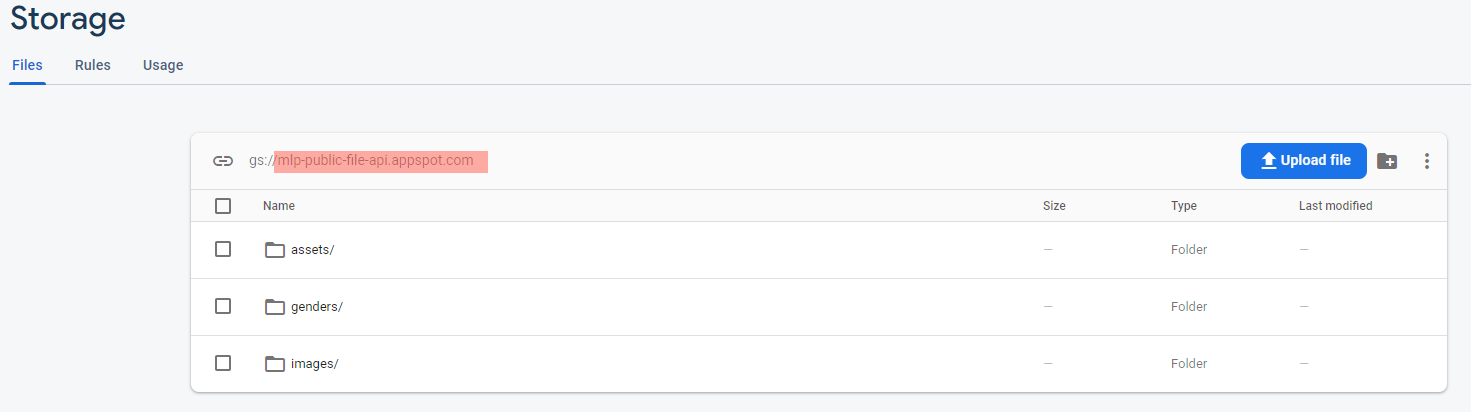
\includegraphics[width=\textwidth]{firebase_storage_bucket}
    \caption{Пример страницы Firebase Storage проекта}\label{fig:firebase_storage_bucket}
\end{figure}


\subsection{Сервис уведомлений}

Сервис уведомлений это консольное .NET приложение. Он обрабатывает сообщения из очереди RabbitMQ и на их основе отправляет уведомления пользователям.

Запуск сервиса происходит через powershell консоль. Сборка и запуск сервиса через powershell консоль:

\begin{lstlisting}[language=bash]
dotnet run --project .\TwilightSparkle.NotificationService.csproj
\end{lstlisting}

Для остановки сервиса также достаточно закрыть окно консоли или остановить выполнение комбинацией клавиш Ctrl и C.

\bigskip
\textbf{Сборка сервиса}

Для перехода в папку сервиса управления проектами используем:

\begin{lstlisting}[language=bash]
cd \notification-service\src
\end{lstlisting}

Сборка проекта и проверка его работоспособности через запуск exe файла:

\begin{lstlisting}[language=bash]
cd \TwilightSparkle.NotificationService
dotnet build --project .\TwilightSparkle.NotificationService.csproj
cd \bin\Debug\net5.0
.\TwilightSparkle.NotificationService.exe
\end{lstlisting}

\bigskip
\textbf{Запуск сервиса}

Запуск сервисов, к которым должно вестись подключение, происходит также как и для сервиса развития персонала или сервиса управления проектами.

Для запуска сервиса уведомлений достаточно запустить exe файл, полученный после сборки:

\begin{lstlisting}[language=bash]
cd \TwilightSparkle.NotificationService\bin\Debug\net5.0
.\TwilightSparkle.NotificationService.exe
\end{lstlisting}

Работать с файлом конфигураций нужно также как и в других .NET сервисах.


\subsection{Клиентское приложение}

Клиентское приложение написано на Vue.js и предоставляет UI пользователям программного средства.

\bigskip
\textbf{Настройка клиентского приложения}

Для перехода в папку клиентского приложения используем:

\begin{lstlisting}[language=bash]
cd \client-app\src
\end{lstlisting}

Для настройки проекта:
\begin{lstlisting}[language=bash]
npm install
\end{lstlisting}

\bigskip
\textbf{Запуск клиентского приложения}

Ддя работы клиентского приложения необходимо запустить все .NET Web API сервисы. Их сборка и запуск подробно описан выше.

Для запуска используем:
\begin{lstlisting}[language=bash]
npm run serve
\end{lstlisting}

Для остановки необходимо использовать комбинацию клавиш Ctrl и C.

Таким образом, описаны способы сборки и запуска всех сервисов и клиентского приложения. Данные способы могут быть использованы для любой машины, которую поддерживает программное средство.